\section{La fibre optique}
Les communications optiques existaient déjà du temps des amérindiens avec
l'utilisation des signaux de fumée ! En 1794, le télégraphe optique de Chappe
fait son apparition. Les sémaphores étaient relativement espacés (10 à 30\,km)
et permettaient de transmettre des messages dans toute la France en quelques
heures (en 1844, il existe 5000\,km de lignes Chappe avec 534 stations
permanentes en France ; Paris--Lille : 9 minutes !). Le développement de
l'électricité fait disparaître l'optique des télécommunications avec la mise au
point en 1855 du télégraphe électrique qui permet de communiquer par
l'intermédiaire de fils métalliques, de jour comme de nuit et quelles que soient
les conditions climatiques. L'optique réapparaît vers les années 60 avec
l'apparition du laser (1960). Cependant, un faisceau lumineux qui se propage en
espace libre subit bon nombre de modifications et ce pour diverses raisons :
variation de l'indice de réfraction du chemin traversé par la lumière modifiant
perpétuellement le chemin optique vu par la lumière (variation des conditions
climatiques influant sur l'indice) ; variation de l'atténuation du milieu en
fonction des conditions atmosphériques ; diffraction d'un faisceau lumineux dont
le diamètre transverse $D$ n'est pas infini. Il subit une divergence naturelle
de l'ordre de $\theta = 10^{-4}$\,radian pour un faisceau de $D = 5$\,mm de
diamètre et une longueur d'onde de l'ordre de $\lambda \approx 0.5\,\mu$m. Il en
résulte, après une propagation sur une distance $L$, un élargissement
$\Delta D \approx L\theta$. Par exemple, pour $L = 1$\,km, l'élargissement du
faisceau est de 10\,cm. Il y a donc dispersion de l'énergie par diffraction !

Tout ceci met donc rapidement en évidence la nécessité d'une propagation guidée.
La fibre optique pour la propagation longue distance est mise au point en 1966.
La longueur totale du réseau français dépasse les quelques dizaines de millions
de kilomètres quand le réseau japonais, le plus long du monde, atteignait déjà
en 2010 plus de 110 millions de kilomètres. Débits actuels : 100\,Gb/s par
longueur d'onde installée (500\,Gb/s par longueur d'onde en laboratoire) ;
jusqu'à 88 canaux (one channel per longueur d'onde), soit quelques dizaines de Tb/s sur une fibre optique !\\

This chapter guides the light three times over, the first time by réflexion
totale interne. Après avoir présenté le guidage de la lumière dans un guide
d'onde par l'intermédiaire de l'optique géométrique, nous essayerons de
comprendre, à l'aide de l'optique ondulatoire, pourquoi certaines trajectoires
sont permises alors que d'autres ne le sont pas. Cela permettra d'aborder la
notion de mode transverse, de guide monomode ou multimode, etc. Enfin, nous
montrerons qu'il existe des outils puissants, à partir des équations de
Maxwell, qui permettent de décrire parfaitement la répartition transverse
d'énergie dans un guide aussi bien planaire qu'à symétrie de révolution.

\subsection{Notion de guide d'onde}

\begin{definition}[Guide d'onde optique]
  Un \textbf{guide d'onde} (\textit{waveguide}) optique est une structure
  diélectrique, uniforme le long d'un axe, capable de transporter de l'énergie
  électromagnétique à des longueurs d'onde situées dans les parties infrarouge
  et visible du spectre sur des distances grandes devant la longueur d'onde.
\end{definition}

Un diélectrique est un matériau qui ne possède pas de charges électriques
susceptibles de se déplacer de façon macroscopique. Ainsi, ce milieu ne conduit
pas le courant, il est isolant.\\

Dans la pratique, un guide d'onde dans le domaine optique du spectre est
constitué d'une région diélectrique planaire ou linéaire appelée
\textbf{cœur} (\textit{core}). Cette zone est entourée par un ou plusieurs
milieux diélectriques dont les indices de réfraction sont \emph{inférieurs} à
celui du cœur afin d'assurer le confinement de l'onde. Cette zone extérieure au
cœur est appelée la \textbf{gaine} (\textit{cladding}) du guide. Le cœur de
tous ces guides est l'endroit où l'énergie se propage.\\

Three geometries matter. Le guide le plus simple est le \textbf{guide d'onde
plan à saut d'indice} (\textit{plane step-index guide}) dont la dimension
suivant $y$ est infinie. Le terme « \textbf{saut d'indice} »
(\textit{step index}) signifie que l'indice est constant dans chaque domaine.
La lumière est guidée suivant l'axe $z$. Le guide rectangulaire ou
\textbf{guide à ruban} (\textit{ribbon guide}) se rencontre dans les lasers à
semi-conducteurs produits à des milliards d'exemplaires. Très compliqué, ce
guide ne sera pas étudié ici. Enfin, la fibre est un guide à symétrie de
révolution. Son étude se rapproche de celle du guide plan mais s'avère plus
complexe.

\begin{remark}
  Les méthodes numériques utilisées pour résoudre le problème de la
  propagation dans un guide diélectrique sont souvent compliquées. Nous nous
  contenterons d'analyser le guide planaire à saut d'indice. Bien que son étude
  revêt clairement un aspect idéal (dimension infinie suivant $y$), il permet
  de comprendre la plupart des mécanismes de guidage de la lumière et les
  problématiques liées au confinement de cette dernière. C'est ce guide que
  nous utiliserons lors des deux prochaines parties : approche géométrique et
  approche ondulatoire.
\end{remark}

\paragraph{Dimension typique d'une fibre} Les caractéristiques typiques d'une
fibre optique sont
\[
  n_{\text{verre}} \approx 1.44\text{--}1.46, \qquad
  \Delta n = n_{\text{cœur}} - n_{\text{gaine}} = 10^{-3}\ \text{to}\ 2\times 10^{-2},
  \qquad D_{\text{cœur}} = 2a = 5\ \text{to}\ 50\,\mu\mathrm{m}.
\]
La fibre la plus utilisée dans le domaine des télécommunications optiques
haut-débit est la fibre dite monomode standard SMF28 (\textit{Single Mode
Fiber}). Ses diamètres typiques sont $D_{\text{cœur}} =
9\,\mu$m et $D_{\text{gaine}} = 125\,\mu$m; the gaine is itself protected by a
polymer coating taking the outer diameter to
$250\,\mu$m. Cette enveloppe protectrice supplémentaire assure une protection à
la fois mécanique et surtout optique vis à vis de la lumière extérieure mais ne
participe pas au guidage. Le diélectrique utilisé est dans la plupart des cas
de la silice dopée par du bore, qui facilite la fusion du verre, empêche la
dévitrification et améliore la résistance à l'eau, et par du germanium
($n_{\text{Ge}} \approx 4.2$ à $1550$\,nm et $300$\,K), qui permet suivant sa
concentration d'augmenter l'indice du verre. D'autres ingrédients sont
également utilisés. Cette cuisine relève souvent du secret industriel dans un
domaine qui est très concurrentiel.

\subsection{Approche géométrique du guidage}

\subsubsection{Rappel de la notion de réflexion totale}
Il est courant de représenter la lumière par des « rayons lumineux ». Cette
représentation est le fruit d'une approximation : la longueur d'onde de l'onde
monochromatique représentée est petite devant les structures dans lesquelles
elle se propage. Dans ce cas, on définit les rayons comme les courbes normales
aux surfaces équiphases ou fronts d'onde. Les lois de la réflexion et de la
réfraction pour les ondes planes à l'interface entre deux milieux s'appliquent
aux rayons.

Si on reprend le cas d'un faisceau traversant un dioptre, d'un milieu
\emph{plus} réfringent vers un milieu \emph{moins} réfringent (du cœur vers la
gaine), on constate que le faisceau s'écarte de la normale. De plus, on
constate que pour une certaine valeur de $i$ appelée angle limite $i_c$, le
faisceau réfracté est perpendiculaire à l'axe $x$ ($i' = 90^\circ$) ! Seul le
rayon réfléchi existe, le faisceau réfracté n'existe plus. On parle alors de
réflexion totale ! Inside a guide, from cœur to gaine, this is
\textbf{réflexion totale interne} (\textit{total internal reflection}, RTI).

L'angle limite se détermine d'après la loi de Descartes-Snell,
\begin{equation*}
  n_c \sin i = n_g \sin i',
\end{equation*}
en se plaçant dans le cas de la réflexion totale ($i' = 90^\circ$) :
\begin{equation*}
  i_c = \sin^{-1}\!\left(\frac{n_g}{n_c}\right)
  \qquad\text{and}\qquad
  \frac{\theta_c}{2} = \frac{\pi}{2} - i_c = \cos^{-1}\!\left(\frac{n_g}{n_c}\right).
\end{equation*}

\begin{prop}[Condition de réflexion totale]
  Pour avoir réflexion totale, il faut que $i > i_c$ --- equivalently
  $\theta/2 < \theta_c/2$, where $\theta/2$ is the angle the ray makes with the
  guide axis $z$.
\end{prop}

\begin{example}[Application numérique]
  Soit $n_c = 1.46$ et
  $\Delta = (n_c - n_g)/n_c = 0{,}34\%$, the relative index difference. Alors,
  $n_g = 1.455$. On a alors :
  \[
    i_c = 85{,}3^\circ \qquad\text{or}\qquad \frac{\theta_c}{2} = 4{,}7^\circ .
  \]
  The whole guiding business plays out inside a cone less than five degrees
  wide about the axis.
\end{example}

\subsubsection{Guidage de la lumière par réflexion totale interne}
On enferme un milieu d'indice $n_c$ entre 2 milieux d'indice plus faible $n_g$.
Si l'angle du faisceau $\theta/2$ est inférieur à $\theta_c/2$, le faisceau se
retrouve confiné dans le cœur par réflexion totale sur les interfaces
cœur/gaine. On parle alors de guidage par réflexion totale interne (RTI). Si le
faisceau incident est injecté avec un angle trop important dans la fibre, en
dehors du \textbf{cône d'acceptance} (\textit{acceptance cone}) --- of opening
angle $\alpha$ ---, le faisceau ne sera pas complètement réfléchi et finira par
s'atténuer irrémédiablement au fur et à mesure de la propagation. Ce faisceau
n'est donc pas guidé ! That $\alpha$ spans the whole cone, from the highest
accepted ray to the lowest; the half-angle measured from the axis --- the
maximum incidence in air --- is written $i_0$.

\begin{figure}[h!]
  \centering
  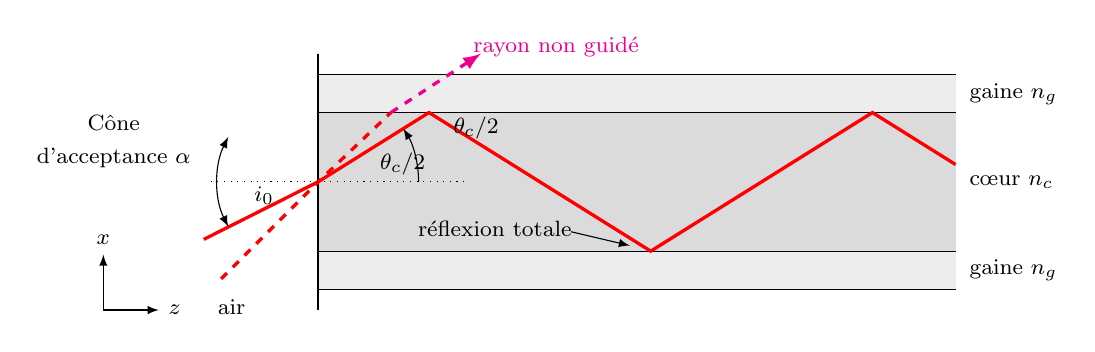
\begin{tikzpicture}[>=latex,scale=0.88]
    % cladding
    \fill[black!7] (1.2,1) rectangle (10.4,1.55);
    \fill[black!7] (1.2,-1.55) rectangle (10.4,-1);
    % core
    \fill[black!14] (1.2,-1) rectangle (10.4,1);
    \draw (1.2,1) -- (10.4,1);
    \draw (1.2,-1) -- (10.4,-1);
    \draw (1.2,1.55) -- (10.4,1.55);
    \draw (1.2,-1.55) -- (10.4,-1.55);
    % input face
    \draw[thick] (1.2,-1.85) -- (1.2,1.85);
    % guided ray
    \draw[very thick,red] (1.2,0) -- (2.8,1) -- (6.0,-1) -- (9.2,1) -- (10.4,0.25);
    % incoming ray inside the acceptance cone
    \draw[very thick,red] (-0.45,-0.83) -- (1.2,0);
    % non guided ray
    \draw[very thick,red,dashed] (-0.2,-1.4) -- (1.2,0) -- (2.25,1);
    \draw[very thick,magenta,dashed,->] (2.25,1) -- (3.55,1.85);
    % acceptance cone
    \draw[<->] ([shift=(206.6:1.45)]1.2,0) arc (206.6:153.4:1.45);
    \draw[dotted] (-0.35,0) -- (3.3,0);
    \node[align=center] at (-1.75,0.58)
      {\footnotesize Cône\\ \footnotesize d'acceptance $\alpha$};
    \node at (0.42,-0.2) {\footnotesize $i_0$};
    % labels
    \draw[->] ([shift=(0:1.45)]1.2,0) arc (0:32:1.45);
    \node at (2.42,0.26) {\footnotesize $\theta_c/2$};
    \node at (3.48,0.78) {\footnotesize $\theta_c/2$};
    \node[right] at (10.46,1.27) {\footnotesize gaine $n_g$};
    \node[right] at (10.46,0) {\footnotesize cœur $n_c$};
    \node[right] at (10.46,-1.27) {\footnotesize gaine $n_g$};
    \node at (-0.05,-1.8) {\footnotesize air};
    \node[magenta,right] at (3.3,1.95) {\footnotesize rayon non guidé};
    \node at (3.75,-0.68) {\footnotesize réflexion totale};
    \draw[->] (4.85,-0.72) -- (5.7,-0.92);
    % axes
    \draw[->] (-1.9,-1.85) -- (-1.9,-1.05) node[above] {\footnotesize $x$};
    \draw[->] (-1.9,-1.85) -- (-1.1,-1.85) node[right] {\footnotesize $z$};
  \end{tikzpicture}
\end{figure}

\begin{remark}[Ouverture numérique]
  On montre que dans une fibre optique $\theta_{\max} \approx \sqrt{2\Delta}$,
  where $\theta_{\max}$ is the largest angle to the axis $0z$ a ray may make
  \emph{inside} the cœur and still stay guided (it is $\theta_c/2$ to first
  order in $\Delta$). Cette valeur est appelée \textbf{ouverture numérique}
  (\textit{numerical aperture}, ON) --- loosely, since the ouverture numérique
  proper is the sine of the largest incidence in air, which is larger by a
  factor of the index of the cœur.
\end{remark}

\begin{remark}
  Dans un guide plan, les rayons se propagent dans le plan $x$--$z$. Cela
  signifie que l'énergie lumineuse sera effectivement piégée dans la couche
  dans le plan vertical mais \emph{pas} dans le plan horizontal supposé infini
  dans la direction $y$. Le faisceau qu'on injecterait dans un tel guide
  continuerait de s'élargir par diffraction dans le plan de la couche.
\end{remark}

\subsubsection{Profil d'indice}
\begin{definition}[Profil d'indice]
  Le \textbf{profil d'indice} (\textit{index profile}) d'un guide définit la
  variation transverse de l'indice, selon la direction $x$ dans notre cas. Un
  guide est complètement défini par son profil d'indice.
\end{definition}

Le plus simple à fabriquer est le profil à saut d'indice dans lequel la fibre
est constituée de deux zones concentriques homogènes avec un saut brutal
d'indice à l'interface cœur/gaine. De nombreux autres profils existent suivant
les applications visées --- depressed gaine, raised gaine, triangular
cœur. Un exemple de profil d'indice typique, a convenient family covering the
cases of interest, peut être donné par l'expression ci-dessous :
\begin{equation*}
  \begin{cases}
    n^2(x) = n_0^2\left[1 - 2\Delta\left(\dfrac{x}{a}\right)^{\alpha}\right]
      & \text{for } |x| < a,\\[2ex]
    n^2(x) = n_0^2\left[1 - 2\Delta\right] & \text{for } |x| > a,
  \end{cases}
\end{equation*}
avec $\alpha \in \reals^{+}$. On constate que ce profil est de forme
triangulaire si $\alpha = 1$, parabolique si $\alpha = 2$, et à saut d'indice si
$\alpha \rightarrow \infty$.

\begin{figure}[h!]
  \centering
  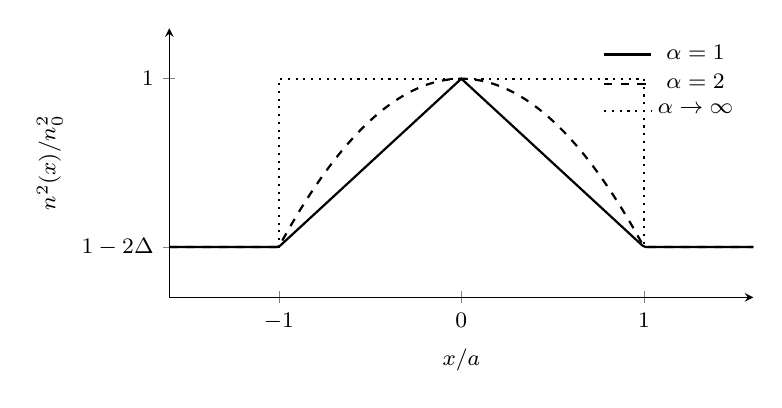
\begin{tikzpicture}
    \begin{axis}[
      width=9cm, height=5cm,
      xlabel={$x/a$}, ylabel={$n^2(x)/n_0^2$},
      xmin=-1.6, xmax=1.6, ymin=0.87, ymax=1.03,
      ytick={0.9,1}, yticklabels={$1-2\Delta$,$1$},
      xtick={-1,0,1}, xticklabels={$-1$,$0$,$1$},
      legend style={at={(0.99,0.98)},anchor=north east,draw=none,fill=none,
                    font=\footnotesize},
      tick label style={font=\footnotesize},
      label style={font=\footnotesize},
      axis lines=left,
      ]
      \addplot[thick,domain=-1.6:1.6,samples=201]{1-0.1*min(abs(x),1)};
      \addlegendentry{$\alpha=1$}
      \addplot[thick,dashed,domain=-1.6:1.6,samples=201]{1-0.1*(min(abs(x),1))^2};
      \addlegendentry{$\alpha=2$}
      \addplot[thick,dotted] coordinates
        {(-1.6,0.9) (-1,0.9) (-1,1) (1,1) (1,0.9) (1.6,0.9)};
      \addlegendentry{$\alpha\rightarrow\infty$}
    \end{axis}
  \end{tikzpicture}
\end{figure}

\noindent (The vertical scale is exaggerated; in a real fibre $2\Delta$ is a
fraction of a percent.) On peut déterminer, par l'approche des rayons, la
trajectoire des rayons lumineux dans la fibre. Cette trajectoire (forme,
période, amplitude…) dépend de nombreux paramètres : profil d'indice transverse
de la fibre, taille transverse du guide, longueur d'onde, angle d'incidence.
Ainsi, on peut trouver des trajectoires en dents de scie dans un guide à saut
d'indice ou des trajectoires sinusoïdales dans un guide à profil parabolique.
Les trajectoires au sein d'un même guide peuvent être multiples dans les guides
multimodes ou unique dans les guides \textbf{monomodes}
(\textit{single-mode}).\\

Le problème est que le temps de trajet dans la fibre dépend de la trajectoire.
Naturellement, s'il existe différentes trajectoires possibles, la lumière
injectée dans la fibre se répartit sur chacune d'entre elles.

\subsubsection{Influence de la dispersion intermodale sur une communication optique}
Une transmission optique numérique consiste à injecter dans la fibre, dans le
cas le plus simple, un signal modulé temporellement en amplitude (ON/OFF).
Après propagation et détection, le signal est remis en forme. Cependant, après
l'injection, la lumière se propage en empruntant les différents chemins
possibles. Après une propagation sur une longueur $L$, l'information qui a
emprunté chaque chemin arrive à des instants différents. Ceci provoque un
élargissement des créneaux. Quand la distance $L$ est trop grande ou le débit
trop important, après remise en forme du signal, celui-ci n'est plus identique
au signal initial, l'information peut être entachée d'erreurs voire
complètement perdue !

\begin{definition}[Dispersion intermodale]
  Ce phénomène de multi-trajets appelé \textbf{dispersion intermodale}
  (\textit{intermodal dispersion}) engendre une limite du débit maximum
  possible --- la \textbf{bande passante} (\textit{bandwidth}) --- sur une
  distance donnée ou réciproquement de la portée de la fibre pour un débit
  donné.
\end{definition}

Si on considère que, pour ne pas commettre d'erreurs à la détection, l'écart
temporel $\Delta\tau$ entre la trajectoire la plus lente et celle la plus rapide
ne doit pas dépasser un quart du \textbf{temps bit} (\textit{bit time})
$T_{\text{bit}}$ avant détection (critère arbitraire --- but a standard one), on
peut en déduire le temps bit minimum (c'est-à-dire la période minimale de
modulation) et donc le débit maximum autorisé sur une fibre :
$T_{\text{bit}} > 4\,\Delta\tau$, soit un \textbf{débit binaire}
(\textit{bit rate}) max acceptable de l'ordre de $1/T_{\text{bit}}$.

\begin{example}[One kilometre of fibre]
  Pour une fibre de $L = 1$\,km,
  \[
    \Delta\tau_{\text{saut d'indice}} = 50\,\mathrm{ns}
    \;\Rightarrow\; T_{\text{bit}} > 200\,\mathrm{ns}
    \;\Rightarrow\; D_{\max} \approx 5\,\mathrm{Mb/s},
  \]
  \[
    \Delta\tau_{\text{parabolique}} = 0{,}25\,\mathrm{ns}
    \;\Rightarrow\; T_{\text{bit}} > 1\,\mathrm{ns}
    \;\Rightarrow\; D_{\max} \approx 1\,\mathrm{Gb/s}.
  \]
  More than two orders of magnitude at stake, on nothing but the shape of the
  profil d'indice.
\end{example}

\begin{remark}[Orders of magnitude]
  Over 1\,km the spread for a saut d'indice profile is
  $\Delta\tau_{\text{saut d'indice}} = 50$\,ns,
  hence $D_{\max} \approx 5$\,Mb/s, while the parabolic profile gives
  $0{,}25$\,ns and $1$\,Gb/s. The ratio of roughly $200$ between the two
  profiles, and the orders of magnitude ``tens of ns'' against ``a fraction of
  a ns'', are what matter in this course.
\end{remark}

\paragraph{Solutions pour s'affranchir de la dispersion intermodale} There are
two.

La première est de modifier le profil d'indice, par exemple en utilisant un
profil à \textbf{gradient d'indice} (\textit{graded index}) où l'indice décroît
au fur et à mesure que l'on s'éloigne du centre de la fibre. La vitesse de la
lumière étant inversement proportionnelle à l'indice de réfraction, le signal
s'accélère lorsque le rayon s'éloigne du centre. Ainsi, bien que les rayons de
plus grande inclinaison aient des trajectoires physiques plus longues, ils se
déplacent plus vite en dehors du centre de la fibre que pour une fibre à saut
d'indice, ce qui réduit la différence de temps de trajets entre les
trajectoires les plus longues et la trajectoire la plus courte. L'influence de
la dispersion modale s'en trouve réduite.\\

La deuxième solution est de limiter le nombre de trajectoires en fabriquant une
fibre monomode où une seule trajectoire --- la plus rapide ! --- est permise.
La suite explique ce qu'est un mode, son lien avec la trajectoire dans la fibre
et comment en limiter le nombre.

\subsection{Notion de mode transverse par approche interférentielle}

Jusqu'à présent, nous avons raisonné avec une approche géométrique. Cependant,
nous avons omis l'aspect ondulatoire de la lumière. Or, puisque des faisceaux
se croisent, il y a certainement des interférences. Le but est de déterminer la
répartition d'énergie dans un plan transverse au guide : cette répartition
est-elle uniforme dans le cœur, à l'image de l'indice, ou présente-t-elle des
modulations ? The answer is that parmi toutes les trajectoires décrites
précédemment, seules certaines sont permises. Les autres sont interdites et ne
se propagent pas. \emph{Les angles permis sont donc quantifiés.}

\subsubsection{Guide plan idéal : guide composé de deux miroirs plans sans pertes}
Three simplifying hypotheses. First, une fibre à symétrie de révolution
engendre des calculs relativement compliqués, et les trajectoires peuvent
potentiellement être hélicoïdales suivant la manière dont on y injecte la
lumière --- des \textbf{rayons hélicoïdaux} (\textit{helical rays}). Nous nous
limiterons à l'étude des \textbf{rayons méridiens} (\textit{meridional rays}),
un rayon méridien étant confiné sur un plan méridien à l'intérieur d'un
cylindre dont le diamètre est celui du cœur ; pour le guide plan, nous nous
limiterons donc aux rayons dans le plan $x$--$z$. Second, nous allons étudier
la propagation d'une onde entre deux miroirs plans, infinis suivant la
direction $y$, séparés d'une distance $D_{\text{cœur}} = 2a$, supposés sans
pertes. Third, on associe à chaque rayon lumineux une onde électromagnétique
transverse plane (TEM selon la direction du rayon). Le champ électromagnétique
total est la somme de ces ondes planes. L'onde est polarisée dans la direction
$y$ et son vecteur d'onde reste dans le plan $x$--$z$.

Un rayon de lumière faisant un angle $\theta/2$ avec le miroir supérieur se
réfléchit puis se propage avec un angle $-\theta/2$ jusqu'au miroir inférieur,
puis se réfléchit, etc. Puisque le vecteur champ électrique est parallèle aux
miroirs, chaque réflexion s'accompagne d'un déphasage $\pi$ pour un miroir
parfait, sans que ni l'amplitude, ni la polarisation ne varient. (The $\pi$ is
dropped in without proof here: un véritable parachutage ! Les plus curieux iront regarder dans la littérature la notion de facteur de
réflexion de Fresnel.)

\subsubsection{Interférences dans le guide : condition de guidage idéale dans un guide plan à miroir parfait}
Si deux ondes cohérentes se superposent en phase, elles s'ajoutent. Par contre,
si elles sont en opposition de phase, elles se soustraient, générant des
interférences destructives et donc de l'obscurité. Si on reprend le modèle de
la propagation des rayons par réflexion totale interne, dans une approche
ondulatoire, on peut remplacer les rayons par des ondes planes. Elles sont
représentées par des traits parallèles, perpendiculaires à la direction de
propagation, qui représentent les plans équiphases. Le principe du guidage de la lumière est que son énergie
doit rester confinée dans le cœur et se conserver lors de la propagation. Ce
qui revient à considérer que l'onde après deux réflexions doit être en phase
avec l'onde initiale modulo $2\pi$ pour rester en interférence constructive et
continuer de se propager.

\begin{figure}[h!]
  \centering
  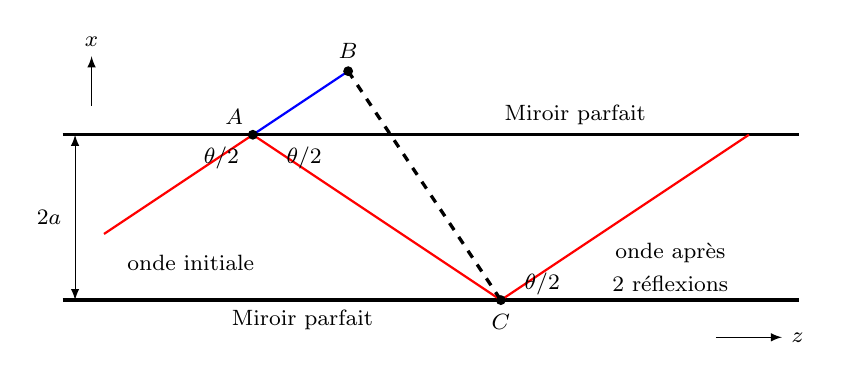
\begin{tikzpicture}[>=latex,scale=1.05]
    % mirrors
    \draw[very thick] (-0.3,1) -- (8.6,1);
    \draw[very thick] (-0.3,-1) -- (8.6,-1);
    \node[above] at (5.9,1) {\footnotesize Miroir parfait};
    \node[below] at (2.6,-1) {\footnotesize Miroir parfait};
    % core width arrow
    \draw[<->] (-0.15,-1) -- (-0.15,1);
    \node[left] at (-0.2,0) {\footnotesize $2a$};
    % initial ray up to A, A to C, C onwards
    \draw[thick,red] (0.2,-0.20) -- (2,1);
    \draw[thick,red] (2,1) -- (5,-1);
    \draw[thick,red] (5,-1) -- (8,1);
    % wavefront BC
    \draw[very thick,dashed] (3.153,1.769) -- (5,-1);
    % AB segment
    \draw[thick,blue] (2,1) -- (3.153,1.769);
    % points
    \fill (2,1) circle (1.7pt);      \node[above left] at (2,1) {\footnotesize $A$};
    \fill (3.153,1.769) circle (1.7pt); \node[above] at (3.153,1.8) {\footnotesize $B$};
    \fill (5,-1) circle (1.7pt);     \node[below] at (5,-1.05) {\footnotesize $C$};
    % angles
    \node at (1.62,0.72) {\footnotesize $\theta/2$};
    \node at (2.62,0.72) {\footnotesize $\theta/2$};
    \node at (5.5,-0.8) {\footnotesize $\theta/2$};
    % annotations
    \node[align=center] at (7.05,-0.6)
      {\footnotesize onde après\\ \footnotesize 2 réflexions};
    \node at (1.25,-0.55) {\footnotesize onde initiale};
    \draw[->] (7.6,-1.45) -- (8.4,-1.45) node[right] {\footnotesize $z$};
    \draw[->] (0.05,1.35) -- (0.05,1.95) node[above] {\footnotesize $x$};
  \end{tikzpicture}
\end{figure}

En termes de déphasage, counting the two reflections as $-2\pi$,
\begin{equation*}
  \Delta\varphi = \frac{2\pi}{\lambda}\,n_c\,(AC - AB) - 2\pi = 2\pi q,
  \qquad q = 0,1,2,3,\dots
\end{equation*}
Ainsi, les deux ondes se séparant au point $A$ doivent chacune avoir parcouru
des chemins optiques jusqu'aux points $B$ et $C$ tels que leur différence doit
être un multiple de la longueur d'onde :
\begin{equation*}
  n_c\,(AC - AB) = (q+1)\lambda = m\lambda, \qquad m = 1,2,3,\dots
\end{equation*}
With $a$ the half-width of the guide, trigonometry gives
\begin{equation*}
  AB = AC\cos\theta \qquad\text{and}\qquad AC = \frac{2a}{\sin\theta/2},
\end{equation*}
and there remains the \textbf{condition de guidage} (\textit{guiding
condition}) itself.

\begin{theorem}[Condition de guidage idéale dans un guide plan à miroir parfait]
  \begin{equation*}
    D_{\text{cœur}} = 2a = m\,\frac{\lambda}{2n_c\sin\dfrac{\theta}{2}},
    \qquad m = 1,2,3,\dots
  \end{equation*}
\end{theorem}

Cette condition de guidage relie les paramètres physiques du guide (diamètre,
indice) aux paramètres de l'onde y circulant (longueur d'onde et angle). Cette
équation peut être vue de différentes manières : pour un guide donné ($n_c$ et
$a$ fixés), on peut étudier pour une longueur d'onde donnée quels sont les
angles permis dans le guide ; pour un guide donné, on peut étudier quelles
longueurs d'onde sont permises dans le guide ; on peut enfin choisir
\emph{a priori} les modes et les longueurs d'onde que l'on souhaite voir se
propager dans le guide et fabriquer la fibre en fonction.

\subsubsection{Modes guidés = angles permis et quantifiés}
Prenons le cas d'une lumière monochromatique de longueur d'onde $\lambda$ se
propageant dans la fibre. Dans l'expression de la condition de guidage, on
constate que pour $a$, $n_c$ et $\lambda$ fixés, il existe un angle donné
$\theta_m$ pour chaque entier $m$ pour que la condition de guidage soit
satisfaite :
\begin{equation*}
  \boxed{\;\frac{\theta_m}{2}
    = \sin^{-1}\!\left(m\,\frac{\lambda}{2 D_{\text{cœur}} n_c}\right)\;}
\end{equation*}

\begin{conclusion}
  Les angles des rayons dont l'énergie est guidée sont \emph{quantifiés}.
  Seuls certains sont permis. Les autres ne se propagent pas, \emph{même s'ils
  satisfont la condition de réflexion totale interne}. Un \textbf{mode guidé}
  (\textit{guided mode}) correspond donc à un angle de propagation dans le
  guide.
\end{conclusion}

\begin{example}[Application numérique]
  Prenons un guide de rayon $a = 4{,}5\,\mu$m (soit $D_{\text{cœur}} =
  9\,\mu$m) dans lequel se propage une lumière de longueur d'onde
  $\lambda = 1{,}55\,\mu$m :
  \[
    \begin{array}{llll}
      m = 1: & \theta_1/2 = 3{,}38^\circ \qquad&
      m = 2: & \theta_2/2 = 6{,}77^\circ \\
      m = 3: & \theta_3/2 = 10{,}19^\circ \qquad&
      m = 4: & \theta_4/2 = 13{,}64^\circ \\
      m = 5: & \theta_5/2 = 17{,}15^\circ &&
    \end{array}
  \]
  Il est également important de noter que chaque angle dépend de $\lambda$.
\end{example}

\begin{remark}[Checking the list]
  Each entry is the boxed formula evaluated directly: for $m = 1$ it gives
  $\theta_1/2 = 3{,}38^\circ$, and the later angles stay close to whole
  multiples of it, the sine being still nearly linear at these angles.
\end{remark}

\subsubsection{Distribution transverse d'intensité}
Pour un angle donné, des ondes vont se propager à la fois vers le haut avec un
angle $\theta$ et vers le bas avec un angle $-\theta$ et vont donc se croiser.
Ces ondes issues de la même source sont cohérentes et vont donc interférer. Le
déphasage entre les deux ondes planes est
\begin{equation*}
  \Delta\varphi = \varphi_2 - \varphi_1
    = \frac{4\pi}{\lambda}\,n_c\,x\,\sin\frac{\theta}{2},
\end{equation*}
et des interférences constructives se forment lorsque $\Delta\varphi$ est un
multiple de $2\pi$. Cette figure d'interférence est constituée de franges
sinusoïdales parallèles au plan $y0z$, elle ne dépend que de $x$, est
indépendante de $y$ et de $z$. Plus l'angle entre les deux ondes est grand,
plus l'interfrange est petit.\\

On pourrait montrer que les angles permis correspondent à des situations où
les interférences sont \emph{destructives sur les miroirs}. S'il n'y a pas
d'énergie aux interfaces, la lumière reste guidée. Sinon, la lumière n'est plus
guidée car une partie de l'énergie fuit dans la gaine au fur et à mesure des
réflexions successives.

\begin{figure}[h!]
  \centering
  \foreach \m in {1,2,3,4}{%
    \begin{tikzpicture}
      \begin{axis}[
        width=4.0cm, height=3.6cm,
        xmin=-1.05, xmax=1.05, ymin=-0.06, ymax=1.15,
        xtick={-1,1}, xticklabels={$-a$,$a$},
        ytick=\empty,
        xlabel={\footnotesize $x$},
        title={\footnotesize $m=\m$},
        tick label style={font=\footnotesize},
        axis lines=left, axis line style={-},
        ]
        \addplot[thick,domain=-1:1,samples=161]
          {sin(\m*90*(x+1))^2};
      \end{axis}
    \end{tikzpicture}\hfill}
\end{figure}

Chaque mode peut être vu comme une onde stationnaire dans la direction $x$, se
propageant dans la direction $z$. Le nombre $m$ représente le nombre de franges
visibles entre les deux miroirs ; on l'appellera l'\textbf{ordre du mode}
(\textit{order of the mode}). La répartition transverse d'intensité suivant $x$
sera donc sinusoïdale dans le cœur, s'annulant sur les miroirs.

\begin{definition}[Mode transverse]
  Un \textbf{mode transverse} (\textit{transverse mode}) guidé correspond à un
  angle de propagation dans le guide \emph{et} une répartition transverse
  donnée. Un mode transverse est un champ qui maintient sa répartition
  transverse et sa polarisation suivant la direction de propagation $z$.
\end{definition}

\begin{remark}
  $m = 0$ ne fournissant pas de solution, il n'est pas permis ! This changes
  once the mirrors are replaced by real dielectric interfaces.
\end{remark}

\subsubsection{Nombre de modes guidés}
Un sinus étant toujours inférieur à $1$, on peut écrire
\begin{equation*}
  \sin\frac{\theta_m}{2} = m\,\frac{\lambda}{2D_{\text{cœur}}n_c} < 1
  \qquad\Longrightarrow\qquad
  m < \frac{2D_{\text{cœur}}n_c}{\lambda},
\end{equation*}
et le nombre de modes guidés peut donc s'écrire
\begin{equation*}
  \boxed{\;m_{\max} \le E\!\left[\frac{2D_{\text{cœur}}n_c}{\lambda}\right]\;}
\end{equation*}
où $E[\,\cdot\,]$ représente la partie entière. Le nombre de modes augmente
avec le rapport $2D_{\text{cœur}}n_c/\lambda$ :
\begin{itemize}
  \item si $2D_{\text{cœur}}n_c/\lambda < 1$, aucun mode ne peut se propager ;
  \item si $1 < 2D_{\text{cœur}}n_c/\lambda < 2$, seul le mode fondamental
    $m = 1$ peut se propager. Le guide est dit monomode transverse.
\end{itemize}

\begin{example}
  Reprenons un guide d'épaisseur $9\,\mu$m dans lequel se propage une lumière
  de longueur d'onde $\lambda = 1{,}55\,\mu$m. Alors, le nombre maximum de
  modes pouvant se propager est $m < 16{,}95$ : seuls $16$ modes peuvent se
  propager dans ce guide \emph{idéal}. Bizarre, le guide n'est pas monomode ---
  yet the SMF28 is supposed to be monomode at that longueur d'onde. The
  perfect-mirror model is missing something, and what it is missing is
  réflexion totale interne.
\end{example}

\subsubsection{Constante de propagation}
\begin{remark}
  \textit{Pour aller plus loin} --- this subsection and the next go beyond the
  main line of this course.
\end{remark}

In the cœur the vecteur d'onde has norm $n_c k_0$, and its component along $x$ is
\begin{equation*}
  k_{xm} = n_c k_0 \sin\!\left(\frac{\theta_m}{2}\right)
         = m\,\frac{\pi}{D_{\text{cœur}}},
  \qquad \|\v{k}_0\| = \frac{2\pi}{\lambda}.
\end{equation*}
Une onde guidée se compose de deux ondes planes distinctes se propageant dans
le plan $x$--$z$, faisant un angle $\pm\theta/2$ avec l'axe $z$. Ses vecteurs
d'onde ont des composantes $(k_x,0,k_z)$ et $(-k_x,0,k_z)$. Leur somme ou leur
différence varie selon $z$ en $\exp(-jk_z z)$. On peut alors dire que la
constante de propagation suivant $z$ d'une onde guidée est
$\gamma \equiv k_z = n_c k_0\cos\theta/2$. Ainsi, $\gamma$ est quantifié :
\begin{equation*}
  \gamma_m = n_c k_0\cos\!\left(\frac{\theta_m}{2}\right),
  \qquad
  \gamma_m^2 = n_c^2 k_0^2\cos^2\!\left(\frac{\theta_m}{2}\right)
             = n_c^2 k_0^2\left(1-\sin^2\!\left(\frac{\theta_m}{2}\right)\right),
\end{equation*}
\begin{equation*}
  \boxed{\;\gamma_m^2 = n_c^2 k_0^2
    - \left(m\,\frac{\pi}{D_{\text{cœur}}}\right)^2\;}
\end{equation*}

\begin{figure}[h!]
  \centering
  \begin{tikzpicture}[>=latex,scale=1.0]
    \draw[->] (0,-0.2) -- (0,2.2) node[above] {\footnotesize $x$};
    \draw[->] (-0.2,0) -- (5.2,0) node[right] {\footnotesize $z$};
    \draw[very thick,red,->] (0,0) -- (4.2,1.7)
      node[above right] {\footnotesize $n_c\v{k}_0$};
    \draw[thick,blue,->] (0,0) -- (0,1.7)
      node[midway,left] {\footnotesize $k_{xm}$};
    \draw[thick,blue,->] (0,0) -- (4.2,0)
      node[midway,below] {\footnotesize $k_z = \gamma$};
    \draw[dashed] (4.2,0) -- (4.2,1.7) -- (0,1.7);
    \draw[->] (1.0,0) arc (0:22:1.0);
    \node at (1.32,0.20) {\footnotesize $\theta_m/2$};
  \end{tikzpicture}
\end{figure}

On constate que $\gamma_m$ varie avec $m$. $\gamma$ étant reliée à la vitesse
de propagation des modes suivant $z$, chaque mode se déplace à une vitesse
différente des autres --- cohérent avec le fait que les longueurs de
trajectoires ne soient pas les mêmes, and the wave-optics face of the
dispersion intermodale.

\subsubsection{Équation de dispersion}
\begin{definition}[Équation de dispersion]
  La relation entre la constante de propagation $\gamma$ et la fréquence
  angulaire $\omega$ est une relation caractéristique importante d'un guide,
  connue sous le nom d'\textbf{équation de dispersion} (\textit{dispersion
  equation}).
\end{definition}
Pour un milieu homogène infini, la relation est simple et s'exprime comme
$\omega = c\gamma/n$, with $n$ the medium's index. Pour le mode $m$ d'un guide
plan à miroir parfait, whose cœur has index $n_c$,
\begin{equation*}
  \gamma_m^2 = \frac{n_c^2\omega^2}{c^2}
    - \left(m\,\frac{\pi}{D_{\text{cœur}}}\right)^2 .
\end{equation*}
Pour le guide diélectrique, et \emph{a fortiori} pour la fibre optique à
symétrie de révolution, cette équation de dispersion (et donc sa résolution)
est beaucoup plus complexe et n'admet pas de solution analytique.

\subsection{Guide plan diélectrique}

On considère cette fois un \textbf{guide plan diélectrique} (\textit{dielectric
plane guide}), c'est-à-dire un milieu d'indice $n_c$ entouré par un milieu
d'indice $n_g$. La réflexion a donc lieu sur les dioptres cœur/gaine et non plus
sur des miroirs parfaits.

\subsubsection{Nombre de modes guidés}
À la différence d'un miroir parfait qui réfléchit identiquement quel que soit
l'angle d'incidence, pour un diélectrique, la réflexion dépend de l'angle et il
existe un angle limite pour lequel la réflexion n'est plus totale. Cela
introduit une condition angulaire de guidage par réflexion totale interne, on
top of the interference condition :
\begin{equation*}
  \frac{\theta_m}{2} < \frac{\theta_c}{2}
  = \frac{\pi}{2} - i_c
  = \frac{\pi}{2} - \sin^{-1}\!\left(\frac{n_g}{n_c}\right)
  = \cos^{-1}\!\left(\frac{n_g}{n_c}\right),
\end{equation*}
soit $\sin^{-1}\!\left(m\lambda/2D_{\text{cœur}}n_c\right) <
\cos^{-1}(n_g/n_c)$.

\begin{theorem}[Modes guidés d'un guide plan diélectrique]
  A mode $m$ is guided if and only if
  \begin{equation*}
    m < \frac{2D_{\text{cœur}}n_c}{\lambda}\,
        \sin\!\left(\cos^{-1}\!\left(\frac{n_g}{n_c}\right)\right).
  \end{equation*}
\end{theorem}

Bien que certains modes puissent a priori être guidés dans une structure à
miroirs parfaits, dans un guide diélectrique, si ces modes ne satisfont pas la
condition de réflexion totale, ils s'annulent au fur et à mesure de la
propagation en subissant des pertes à chaque réflexion.

\begin{example}[SMF28 revisited]
  Avec $D_{\text{cœur}} = 9\,\mu$m (dimensions d'une fibre monomode standard
  SMF28) :
  \begin{subpart}
    \item Si $\lambda = 1{,}55\,\mu$m, $m < 1{,}4$ : seul le mode fondamental
      $m = 1$ faisant un angle $\theta_1/2$ par rapport à $z$ est guidé. Le
      guide est dit monomode. Ceci correspond bien à l'application numérique
      précédente où l'on constate que $\theta_2/2 = 6{,}77^\circ$ est
      supérieur à l'angle limite de RTI $\theta_c/2 = 4{,}74^\circ$. Compare
      the perfect-mirror answer, $16$ modes.
    \item Si cette fibre monomode dans l'IR est utilisée dans le violet
      ($\lambda = 0{,}4\,\mu$m), alors $m < 5{,}42$ : 5 modes peuvent se
      propager, les modes $m = 1,2,3,4,5$.
  \end{subpart}
\end{example}

\begin{conclusion}[Ajustement du nombre de modes]
  Pour ajuster le nombre de modes transverses guidés, on peut jouer sur la
  longueur d'onde $\lambda$, la taille de guide $D_{\text{cœur}} = 2a$ et
  l'angle limite $\theta_c/2$ (en jouant sur $n_c$ et $n_g$) : plus
  $\lambda$ diminue, plus $m$ augmente ; plus $D_{\text{cœur}}$ diminue, plus
  $m$ diminue ; plus $\theta_c/2$ diminue, plus $m$ diminue. Donc, pour rendre
  le guide monomode, il faut diminuer la taille du guide ou diminuer
  $\theta_c/2$ (en augmentant $n_g$ par rapport à $n_c$).
\end{conclusion}

\subsubsection{Longueur d'onde de coupure}
On sait que pour qu'un mode soit guidé, il faut remplir la condition
$\theta_m/2 < \theta_c/2$. Read the other way round, pour un mode donné $m$,
dans un guide donné ($a$, $n_c$ et $n_g$ fixés), on peut définir une condition
sur la longueur d'onde pour l'existence d'un mode :
\begin{equation*}
  \boxed{\;\lambda < \lambda_{cm}
    = \frac{2D_{\text{cœur}}n_c}{m}\,
      \sin\!\left(\cos^{-1}\!\left(\frac{n_g}{n_c}\right)\right)\;}
\end{equation*}

\begin{example}[Application numérique]
  For the same guide,
  \[
    \lambda_{C1} = 2{,}17\,\mu\mathrm{m},\quad
    \lambda_{C2} = 1{,}08\,\mu\mathrm{m},\quad
    \lambda_{C3} = 0{,}72\,\mu\mathrm{m},\quad
    \lambda_{C4} = 0{,}54\,\mu\mathrm{m},\quad
    \lambda_{C5} = 0{,}43\,\mu\mathrm{m}.
  \]
  Le mode $1$ existe si $\lambda < 2{,}17\,\mu$m, le mode $2$ si
  $\lambda < 1{,}08\,\mu$m, etc. Le guide est donc monomode si la longueur
  d'onde $\lambda$ est comprise entre $\lambda_{C2}$ et $\lambda_{C1}$, soit
  \[
    1{,}08\,\mu\mathrm{m} < \lambda < 2{,}17\,\mu\mathrm{m}.
  \]
  Pour $\lambda = 0{,}4\,\mu$m, on retrouve bien que 5 modes se propagent car
  $\lambda < \lambda_{C5}$.
\end{example}

\subsubsection{Correction du modèle utilisé}
Dans le modèle précédent du guide diélectrique, nous avons omis le fait que,
lorsque $n_c > n_g$ et que $\theta/2 < \theta_c/2$, c'est-à-dire que l'on se
place dans le cas de la réflexion totale, la réflexion d'une onde fait
apparaître un déphasage $\varphi_r(\theta/2)$ --- no longer $\pi$ ---
relativement complexe qui dépend de l'angle d'incidence $\theta/2$ \emph{et}
de la polarisation de l'onde (coefficients de Fresnel). Il convient alors de
distinguer deux types de polarisation :
\begin{itemize}
  \item \textbf{Mode TE} (Transverse Électrique) : le champ
    électrique est polarisé perpendiculairement au plan $x$--$z$ ;
  \item \textbf{Mode TM} (Transverse Magnétique) : le champ
    magnétique est polarisé perpendiculairement au plan $x$--$z$.
\end{itemize}
The round-trip phase condition
$\Delta\varphi = (4\pi/\lambda)\,n_c\,x\,\sin(\theta/2) + 2\pi$ devient
\begin{equation*}
  \Delta\varphi = \frac{4\pi}{\lambda}\,n_c\,x\,\sin\frac{\theta}{2}
    + 2\varphi_r\!\left(\frac{\theta}{2}\right) = 2m\pi,
  \qquad m = 0,1,2,3,\dots
\end{equation*}

Three consequences follow. La condition de guidage est alors différente du
guide à miroir parfait et diffère suivant la polarisation étudiée ; elle
aboutit à l'expression d'une \emph{équation transcendante}, appelée équation
de dispersion, qui ne possède pas de solution analytique. La résolution est
numérique ou graphique et permet de trouver les angles permis dans le guide.
Les miroirs n'étant plus parfaits, le champ n'est plus nul aux interfaces : il
est toujours sinusoïdal dans le cœur, mais dans la gaine il prend l'expression
d'une \textbf{onde évanescente} (\textit{evanescent wave}) : le champ décroît
exponentiellement dans la gaine. De plus, contrairement au cas où on ne tient
pas compte de ce déphasage, ici, $m = 0$ est permis. Ceci engendre qu'\emph{il
n'existe pas de longueur d'onde de coupure absolue pour un guide symétrique}.
Le mode $m=0$ se propage toujours. Par contre, $m = 0$ ne correspond pas à
$\theta = 0$ mais au plus petit angle guidé dans le guide.

\begin{figure}[h!]
  \centering
  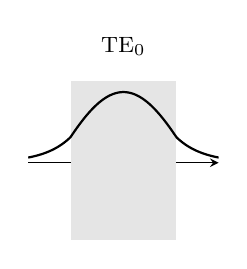
\begin{tikzpicture}
    \begin{axis}[
      width=4.0cm, height=3.6cm,
      xmin=-1.8, xmax=1.8, ymin=-1.1, ymax=1.15,
      xtick=\empty, ytick=\empty,
      title={\footnotesize TE$_0$},
      axis x line=middle, axis y line=none,
      ]
      \fill[black!10] (axis cs:-1,-1.1) rectangle (axis cs:1,1.15);
      \addplot[thick,domain=-1.8:1.8,samples=201]
        {abs(x)<1 ? cos(68.75*x) : 0.362*exp(-2*(abs(x)-1))};
    \end{axis}
  \end{tikzpicture}\hfill
  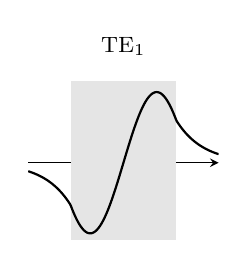
\begin{tikzpicture}
    \begin{axis}[
      width=4.0cm, height=3.6cm,
      xmin=-1.8, xmax=1.8, ymin=-1.1, ymax=1.15,
      xtick=\empty, ytick=\empty,
      title={\footnotesize TE$_1$},
      axis x line=middle, axis y line=none,
      ]
      \fill[black!10] (axis cs:-1,-1.1) rectangle (axis cs:1,1.15);
      \addplot[thick,domain=-1.8:1.8,samples=201]
        {abs(x)<1 ? sin(143.24*x) : ((x>0 ? 0.598 : -0.598)*exp(-2*(abs(x)-1)))};
    \end{axis}
  \end{tikzpicture}\hfill
  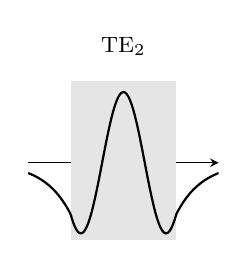
\begin{tikzpicture}
    \begin{axis}[
      width=4.0cm, height=3.6cm,
      xmin=-1.8, xmax=1.8, ymin=-1.1, ymax=1.15,
      xtick=\empty, ytick=\empty,
      title={\footnotesize TE$_2$},
      axis x line=middle, axis y line=none,
      ]
      \fill[black!10] (axis cs:-1,-1.1) rectangle (axis cs:1,1.15);
      \addplot[thick,domain=-1.8:1.8,samples=201]
        {abs(x)<1 ? cos(223.45*x) : -0.726*exp(-2*(abs(x)-1))};
    \end{axis}
  \end{tikzpicture}\hfill
  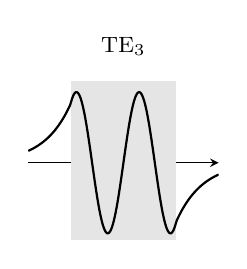
\begin{tikzpicture}
    \begin{axis}[
      width=4.0cm, height=3.6cm,
      xmin=-1.8, xmax=1.8, ymin=-1.1, ymax=1.15,
      xtick=\empty, ytick=\empty,
      title={\footnotesize TE$_3$},
      axis x line=middle, axis y line=none,
      ]
      \fill[black!10] (axis cs:-1,-1.1) rectangle (axis cs:1,1.15);
      \addplot[thick,domain=-1.8:1.8,samples=201]
        {abs(x)<1 ? sin(303.66*x) : ((x>0 ? -0.830 : 0.830)*exp(-2*(abs(x)-1)))};
    \end{axis}
  \end{tikzpicture}
\end{figure}

\noindent The shaded band is the cœur, $|x| < a$. À comparer avec le cas d'un
guide à miroir parfait, where the field is forced to zero exactly on the
mirrors and nothing exists outside the cœur.

\subsection{Résolution formelle à partir des équations de Maxwell}

Si on prend en compte le déphasage à l'interface cœur-gaine pour un guide plan,
le modèle reste complet. Par contre, ce modèle est très difficilement
utilisable dans le cas d'une fibre à symétrie de révolution ! Imaginez les
calculs d'interférences avec des trajectoires hélicoïdales ! Il est
heureusement possible de résoudre ce problème de manière rigoureuse dans le cas
du guide plan aussi bien que dans le cas d'une fibre optique à symétrie de
révolution à partir des équations de Maxwell.

\subsubsection{Cas général}
\begin{postulate}[Les modes propres forment une base]
  L'ensemble des solutions électromagnétiques du problème du guide forme un
  espace vectoriel dont les modes propres forment une base. Une solution
  quelconque pourra donc être représentée comme une combinaison linéaire de
  modes de la structure.
\end{postulate}

Le point de départ est l'équation de propagation pour le champ électrique,
simplifiée parce que l'on considère le milieu diélectrique pur, sans charge ni
courant, mais qui reste valable dans un milieu dont l'indice $n$ varie
lentement sur une longueur égale à la longueur d'onde. Pas de charges :
$\rho = 0$ ; donc, le milieu ne peut générer de courant : $\v{J} = 0$ ; donc sa
conductivité est nulle : $\sigma = 0$. Les équations de Maxwell deviennent
\begin{equation*}
  \begin{cases}
    \curl \v{E} = -\dfrac{\del \v{B}}{\del t}\\[1.6ex]
    \div \v{B} = 0
  \end{cases}
  \qquad
  \begin{cases}
    \curl \v{B} = \varepsilon\mu\dfrac{\del \v{E}}{\del t}\\[1.6ex]
    \div \v{E} = 0
  \end{cases}
\end{equation*}
En éliminant $\v{B}$,
\begin{equation*}
  \curl(\curl \v{E}) = \grad(\div \v{E}) - \Delta \v{E}
    = \varepsilon\mu\frac{\del^2 \v{E}}{\del t^2}
  \qquad\Longrightarrow\qquad
  \varepsilon\mu\frac{\del^2 \v{E}}{\del t^2} - \Delta \v{E} = 0 .
\end{equation*}
Les modes guidés sont les solutions de cette équation, si elles existent, en
forme d'onde progressive le long de l'axe du guide, c'est-à-dire avec une
dépendance en
\begin{equation*}
  \v{E}(\v{r},t) = \v{E}(x)\,e^{i(\omega t - \gamma z)},
\end{equation*}
où $\gamma$ est une quantité a priori inconnue que l'on devra extraire de
l'équation de propagation et qui est appelée constante de propagation (c'est
la même variable que plus haut). Pour une solution sinusoïdale de pulsation $\omega$,
l'équation de propagation devient
\begin{equation*}
  \frac{\del^2 \v{E}(\v{r})}{\del x^2}
  + \frac{\del^2 \v{E}(\v{r})}{\del y^2}
  + \frac{\del^2 \v{E}(\v{r})}{\del z^2}
  + \frac{\omega^2 n^2}{c^2}\,\v{E}(\v{r}) = 0,
\end{equation*}
or, for the plane guide, with the $z$ and $t$ dependence carried by the
exponential,
\begin{equation*}
  \frac{\del^2 \v{E}(x)}{\del x^2}
  + \left(\frac{\omega^2 n^2}{c^2} - \gamma^2\right)\v{E}(x) = 0 .
\end{equation*}
(Il existe les mêmes équations pour le champ magnétique $\v{B}$.) Le principe
est de résoudre cette équation (en coordonnées polaires pour une fibre), dans
les deux régions du guide (cœur et gaine) en établissant des conditions aux
limites qui sont la continuité du champ et de sa dérivée aux interfaces. La
solution générale de l'expression transverse du champ est alors
\begin{equation*}
  \v{E}(x) = \v{A}\,e^{+j\alpha x} + \v{B}\,e^{-j\alpha x},
  \qquad\text{with}\qquad
  \alpha^2 = \frac{\omega^2 n^2}{c^2} - \gamma^2 .
\end{equation*}
En réalité, on cherche un triplet $(\omega,\alpha,\gamma)$ pour lequel
$\v{E}(x)$ est un champ confiné. Pour une fréquence angulaire $\omega$ donnée,
3 cas se présentent car $n$ prend deux valeurs distinctes $n_c$ et $n_g$.

\begin{itemize}
  \item $\gamma > \omega n_c/c > \omega n_g/c$ : $\alpha$ est imaginaire pur et
    le champ est exponentiel dans les trois régions. Pas de réalité physique.
  \item $\omega n_c/c > \gamma > \omega n_g/c$ : le champ est exponentiel
    décroissant dans les régions 1 et 3 et sinusoïdal dans la région 2.
    L'énergie est confinée au voisinage du cœur et fait apparaître une onde
    évanescente dans la gaine.
  \item $\omega n_c/c > \omega n_g/c > \gamma$ : le champ est sinusoïdal dans
    les trois régions. Pas de confinement du champ.
\end{itemize}

\begin{theorem}[Condition d'existence d'un mode guidé]
  La constante de propagation $\gamma$ dans le guide doit être comprise entre
  les deux bornes
  \begin{equation*}
    \frac{\omega n_g}{c} < \gamma < \frac{\omega n_c}{c}
  \end{equation*}
  pour des milieux d'indice $n_g$ et $n_c$ lorsque ces derniers sont illimités.
\end{theorem}

\begin{remark}
  On pourrait montrer que cette condition est identique à la condition de
  réflexion totale $\theta/2 < \theta_c/2$ trouvée précédemment. Cette méthode
  ne permet d'obtenir des solutions analytiques que dans des cas très simples
  (guide plan). Sinon, on doit se contenter d'une résolution graphique pour
  déterminer la valeur de $\gamma$.
\end{remark}

\subsubsection{Résolution dans le cas du guide planaire à saut d'indice}
Dans ce cas, le guide est infini suivant la direction $y$ et l'indice est
constant dans le cœur et dans la gaine. Après quelques simplifications
\[
  \frac{\del}{\del y} = 0 \quad(\text{planar structure}), \qquad
  \frac{\del}{\del z} = -j\beta \quad(\text{propagation along } z), \qquad
  \frac{\del}{\del t} = -j\omega,
\]
on obtient un jeu de 6 équations en $(E_x, E_z, B_y, B_x, B_z, E_y)$. On
constate que les trois premières équations sont indépendantes des 3 dernières.
Les trois premières correspondent au cas TM alors que les 3 dernières
correspondent au cas TE. De ces deux jeux de trois équations, on peut extraire
\begin{equation*}
  \frac{\del^2 E_y(x)}{\del x^2}
    + \left(\frac{\omega^2 n^2}{c^2} - \gamma^2\right) E_y(x) = 0,
  \qquad
  \frac{\del^2 B_y(x)}{\del x^2}
    + \left(\frac{\omega^2 n^2}{c^2} - \gamma^2\right) B_y(x) = 0 .
\end{equation*}
La résolution de ces deux équations et l'application des conditions aux
limites permet de remonter au profil du champ dans le cas TE ou TM, via une
équation de dispersion transcendante comme pour le modèle précédent --- the
corrected interference model. Par exemple, dans le cas TE, on retrouve une
équation de dispersion et une répartition du champ identiques à celles
trouvées dans ce modèle.

\subsubsection{Résolution dans le cas de la fibre}
Pour une fibre à symétrie de révolution, il convient de travailler en
coordonnées polaires. En supposant la continuité de $E$ et de sa dérivée en
$r = a$, si on résout l'équation dans le cas d'une fibre à saut d'indice, on
trouve :
\begin{itemize}
  \item si $r < a$ (cœur), $E$ est une \textbf{fonction de Bessel de première
    espèce} (\textit{Bessel function of the first kind}) ;
  \item si $r > a$ (gaine), $E$ est une \textbf{fonction de Bessel modifiée}
    (\textit{modified Bessel function}).
\end{itemize}
On considère dans un premier temps que le guide est isotrope (invariance par
rotation : pas de différence entre $x$ et $y$). La base de polarisation
linéaire et orthogonale choisie peut être la base $x$ et $y$. Les combinaisons
de modes trouvés sont alors dites de type \textbf{LP} (\textit{Linear
Polarization}) et sont en réalité des solutions approchées.

L'introduction de conditions aux limites fait apparaître une équation de
dispersion, généralement compliquée, qui permet graphiquement de définir
l'existence de telle ou telle solution, comme nous avons pu le constater avec
l'approche géométrique. En réalité, à une dimension (guide plan), le
confinement suivant l'axe $x$ faisait apparaître un et un seul nombre de
quantification $m$. Dans le cas d'une fibre, le confinement est suivant deux
variables, il fait donc apparaître deux nombres quantiques :
\begin{itemize}
  \item suivant le rayon $r$ : confinement à l'intérieur du cœur, un nombre
    quantique $l$ ;
  \item suivant l'angle $\theta$ : après une rotation multiple de $2\pi$, le
    champ doit revenir égal à lui-même, un nombre quantique $m$.
\end{itemize}
Pour $l$ fixé, il existe un nombre fini de solutions de l'équation de
dispersion, $m = 0,1,2,3,\dots$, et le mode correspondant est noté
$\mathrm{LP}_{lm}$. Cette condition d'existence de chaque mode se traduit par
l'apparition de fréquence de coupure comme on l'a vu dans le modèle précédent.
Après injection dans la fibre, la lumière va se répartir suivant les
différents modes pouvant exister (en fonction de la pulsation).

\begin{prop}[Orthogonalité des modes (\textit{orthogonality of the modes})]
  Les modes sont orthogonaux au sens du produit scalaire
  \begin{equation*}
    \int_0^{2\pi}\!\!\int_0^{+\infty}
      \Psi_{lm}\,\Psi^{*}_{l'm'}\;\mathrm{d}r\,\mathrm{d}\theta
    = \begin{cases}
        1 & \text{if } l = l' \text{ and } m = m',\\
        0 & \text{if } l \neq l' \text{ or } m \neq m'.
      \end{cases}
  \end{equation*}
  Un profil d'intensité quelconque se décompose donc sur la base des modes
  propres de la fibre, par exemple
  $a\times \mathrm{LP}_{01} + b\times \mathrm{LP}_{02}
  + c\times \mathrm{LP}_{03}$.
\end{prop}

\begin{remark}[Modes dégénérés]
  Il arrive que l'on puisse avoir deux modes différents avec la même constante
  de propagation $\gamma$. On dit alors qu'ils sont \textbf{dégénérés}
  (\textit{degenerate}). Par exemple, dans une fibre circulaire, une rotation
  de $90^\circ$ autour de l'axe transformera toute solution en une autre
  solution, généralement indépendante de la première mais avec la même
  constante de propagation. Idem pour les solutions paires et impaires, as
  for $\mathrm{LP}_{11}$, $\mathrm{LP}_{12}$, $\mathrm{LP}_{21}$,
  $\mathrm{LP}_{22}$ and $\mathrm{LP}_{31}$.
\end{remark}

\subsection{Performances et domaines d'application}

\begin{conclusion}[Intérêt de la fibre]
  Performance de transmission : très faibles pertes, de l'ordre de
  $0{,}2$\,dB/km ; très grande bande passante, au-delà de $12$\,THz ;
  multiplexage possible sur plusieurs canaux. Mise en œuvre : faible poids,
  faible taille --- gaine de quelques centaines de $\mu$m. Sécurité électrique :
  isolation totale entre terminaux, insensibilité aux parasites électriques
  (n'en crée pas !), possibilité d'utilisation en ambiance explosive,
  applications médicales. Inviolabilité : difficile d'intercepter le signal.
\end{conclusion}

\paragraph{Télécommunications} Il existe près de 300 câbles sous-marins
(environ $885\,000$\,km, $99\%$ des données). Ces câbles font généralement
$8$\,cm de diamètre maximum (pour un poids de $10$\,kg/m), avec plusieurs
fibres par câble fonctionnant par paires (une pour chaque sens de
transmission). Leur débit est proche de $4$\,Tbit/s par paire (200\,000 fois
plus important que le débit d'une connexion ADSL classique).

\paragraph{Imagerie et sources lasers} Imagerie médicale (endoscope, chirurgie
laser) et inspection vidéo ; sources laser de fortes puissances (10\,kW CW),
sources à impulsions ultra-courtes ($< 100$\,fs) et sources larges bandes.

\paragraph{Capteurs distribués} Le principe de base est l'\textbf{OTDR}
(\textit{Optical Time Domain Reflectometer}) : un interrogateur (émission,
détection, traitement des données), and the echo along the fibre locates
events --- a connector, a bend --- by their delay. Two physical effects are
exploited.

In a \textbf{distributed acoustic sensor} (DAS-OTDR), built on Rayleigh
scattering, the pulse illuminates the scattering centres of the $L$th kilometre
of fibre. À un instant donné, on détecte des interférences intra-impulsion à
un endroit :
\begin{equation*}
  I_{\text{rétrodiff}} \;\propto\;
  \left|\sum_i A_i\,e^{j\varphi_i}\right|^2 .
\end{equation*}
Interférences très sensibles au déphasage : pression, déformations, vibrations
de la fibre, ondes acoustiques environnantes. Rappel : diffusion Rayleigh pour
$d \ll \lambda$, diffusion de Mie pour $d \geq \lambda$ ; la diffusion
Rayleigh augmente si $\lambda$ diminue.\\

In \textbf{Brillouin-OTDR} the ambient noise launches an onde acoustique
propagative in the fibre --- apparition d'un réseau d'indice \emph{mobile}, par effet
élasto-optique ($n = f(\text{strain})$). The optical pulse scatters off this
moving grating, and par effet Doppler l'onde est décalée en longueur d'onde:
the measurement is then a spectral analysis. Orders of magnitude: a
pulse $\Delta t = 10$\,ns corresponds to a resolution $\Delta L = 1$\,m, the Raman
shift $\Delta\nu_R$ is a few tens of THz (Raman being sensitive to temperature
alone) and the Brillouin shift is $\Delta\nu_B \approx 11$\,GHz. Rayleigh
scattering, by contrast, is elastic and carries no frequency shift at all,
which is why the DAS-OTDR above reads a phase and the B-OTDR reads a spectrum.\\

Des applications multiples et variées : génie civil et surveillance de la
santé des structures (santé des ouvrages en béton, installation de la fibre
avant coulage), surveillance des fuites et surveillance d'une ville, détection
d'intrusion, ferroviaire et transport (étude du trafic entre deux périodes :
variations du trafic moyen et de la vitesse moyenne), et sismologie --- on
seafloor telecom cables, where it has been used to detect earthquakes and even
ship trajectories.

\paragraph{Autres} Décoration, éclairage ; vêtements ; industrie (marquage par
gravure et frittage, micro-usinage, soudure et perçage de précision, traitement
des matériaux) ; militaire (télémétrie, pointage de cible).
